\documentclass[10pt]{beamer}
\usepackage[utf8]{inputenc}
\usepackage[T1,T2A]{fontenc}
\usepackage[russian]{babel}
\usepackage{color}
\usepackage{calc}
\usepackage{graphicx}
\usepackage{epstopdf}
\usepackage{hyperref}
\hypersetup{unicode,colorlinks}
\usetheme[progressbar=head,numbering=fraction,block=fill]{metropolis}
\usepackage{minted}
\usepackage{dejavu}
%\usepackage{adjustbox}  % Позволяет сузить куски кода (или текст) ровно настолько, чтобы уместиться в слайд
\usepackage{csquotes}
\usepackage{upquote}

\usemintedstyle{solarized-light}
\newminted[haskell]{haskell}{
    escapeinside=!!,
    mathescape=true,
    texcomments=true,
    beameroverlays=true,
    autogobble=true,
    fontsize=\small,
    breaklines=false  % Лучше сам поставлю переносы на удобных местах
}
\newminted[haskellsmall]{haskell}{
    escapeinside=!!,
    mathescape=true,
    texcomments=true,
    beameroverlays=true,
    autogobble=true,
    fontsize=\footnotesize,
    breaklines=false
}
\newminted[haskelltiny]{haskell}{
    escapeinside=!!,
    mathescape=true,
    texcomments=true,
    beameroverlays=true,
    autogobble=true,
    fontsize=\scriptsize,
    breaklines=false
}
\newmintinline[haskinline]{haskell}{
    escapeinside=!!,
    mathescape=true,
    beameroverlays=true,
    breaklines=true
}
\newminted[ghci]{text}{
    autogobble=true,
    fontsize=\small,
    breaklines=false
}
\newminted[ghcismall]{text}{
    autogobble=true,
    fontsize=\footnotesize,
    breaklines=false
}
\newminted[ghcitiny]{text}{
    autogobble=true,
    fontsize=\scriptsize,
    breaklines=false
}
\newmintinline[ghcinline]{text}{
    breaklines=true
}

\newcommand{\hackage}[1]{\href{https://hackage.haskell.org/package/#1}{#1}}

\vfuzz=20pt  % позволяет тексту дойти до номера слайда

\author{Алексей Романов}
\subtitle{Функциональное программирование на Haskell}
%\logo{}
\institute{МИЭТ}
\subject{Функциональное программирование на Haskell}
%\setbeamercovered{transparent}
%\setbeamertemplate{navigation symbols}{}


\title{Лекция 1: введение и основы синтаксиса}
\date{14 февраля 2018}

\begin{document}
\begin{frame}[plain]
\maketitle
\end{frame}

\begin{frame}
\frametitle{Организация курса}
\begin{itemize}
    \item 8 лекций
    \item 4 лабораторных
    \item Итоговый проект
\end{itemize}
\end{frame}

\begin{frame}
\frametitle{Парадигмы программирования}
\begin{itemize}
\item Что такое парадигма?
\pause
\begin{quote}
\enquote{Совокупность идей и понятий, определяющих стиль написания компьютерных программ.} (Wikipedia)
\end{quote}
\pause
\item Основные парадигмы:
\pause
\begin{itemize}
    \item Структурное программирование
    \item Процедурное программирование
    \item \textbf{Функциональное программирование}
    \item Логическое программирование
    \item Объектно-ориентированное программирование
\end{itemize}
\pause
\item В парадигме важно не только то, что используется, но то, использование чего не допускается или минимизируется.
\pause
\item Например, \lstinline!goto! в структурном программировании, глобальные переменные в ООП.
\end{itemize}
\end{frame}

\begin{frame}
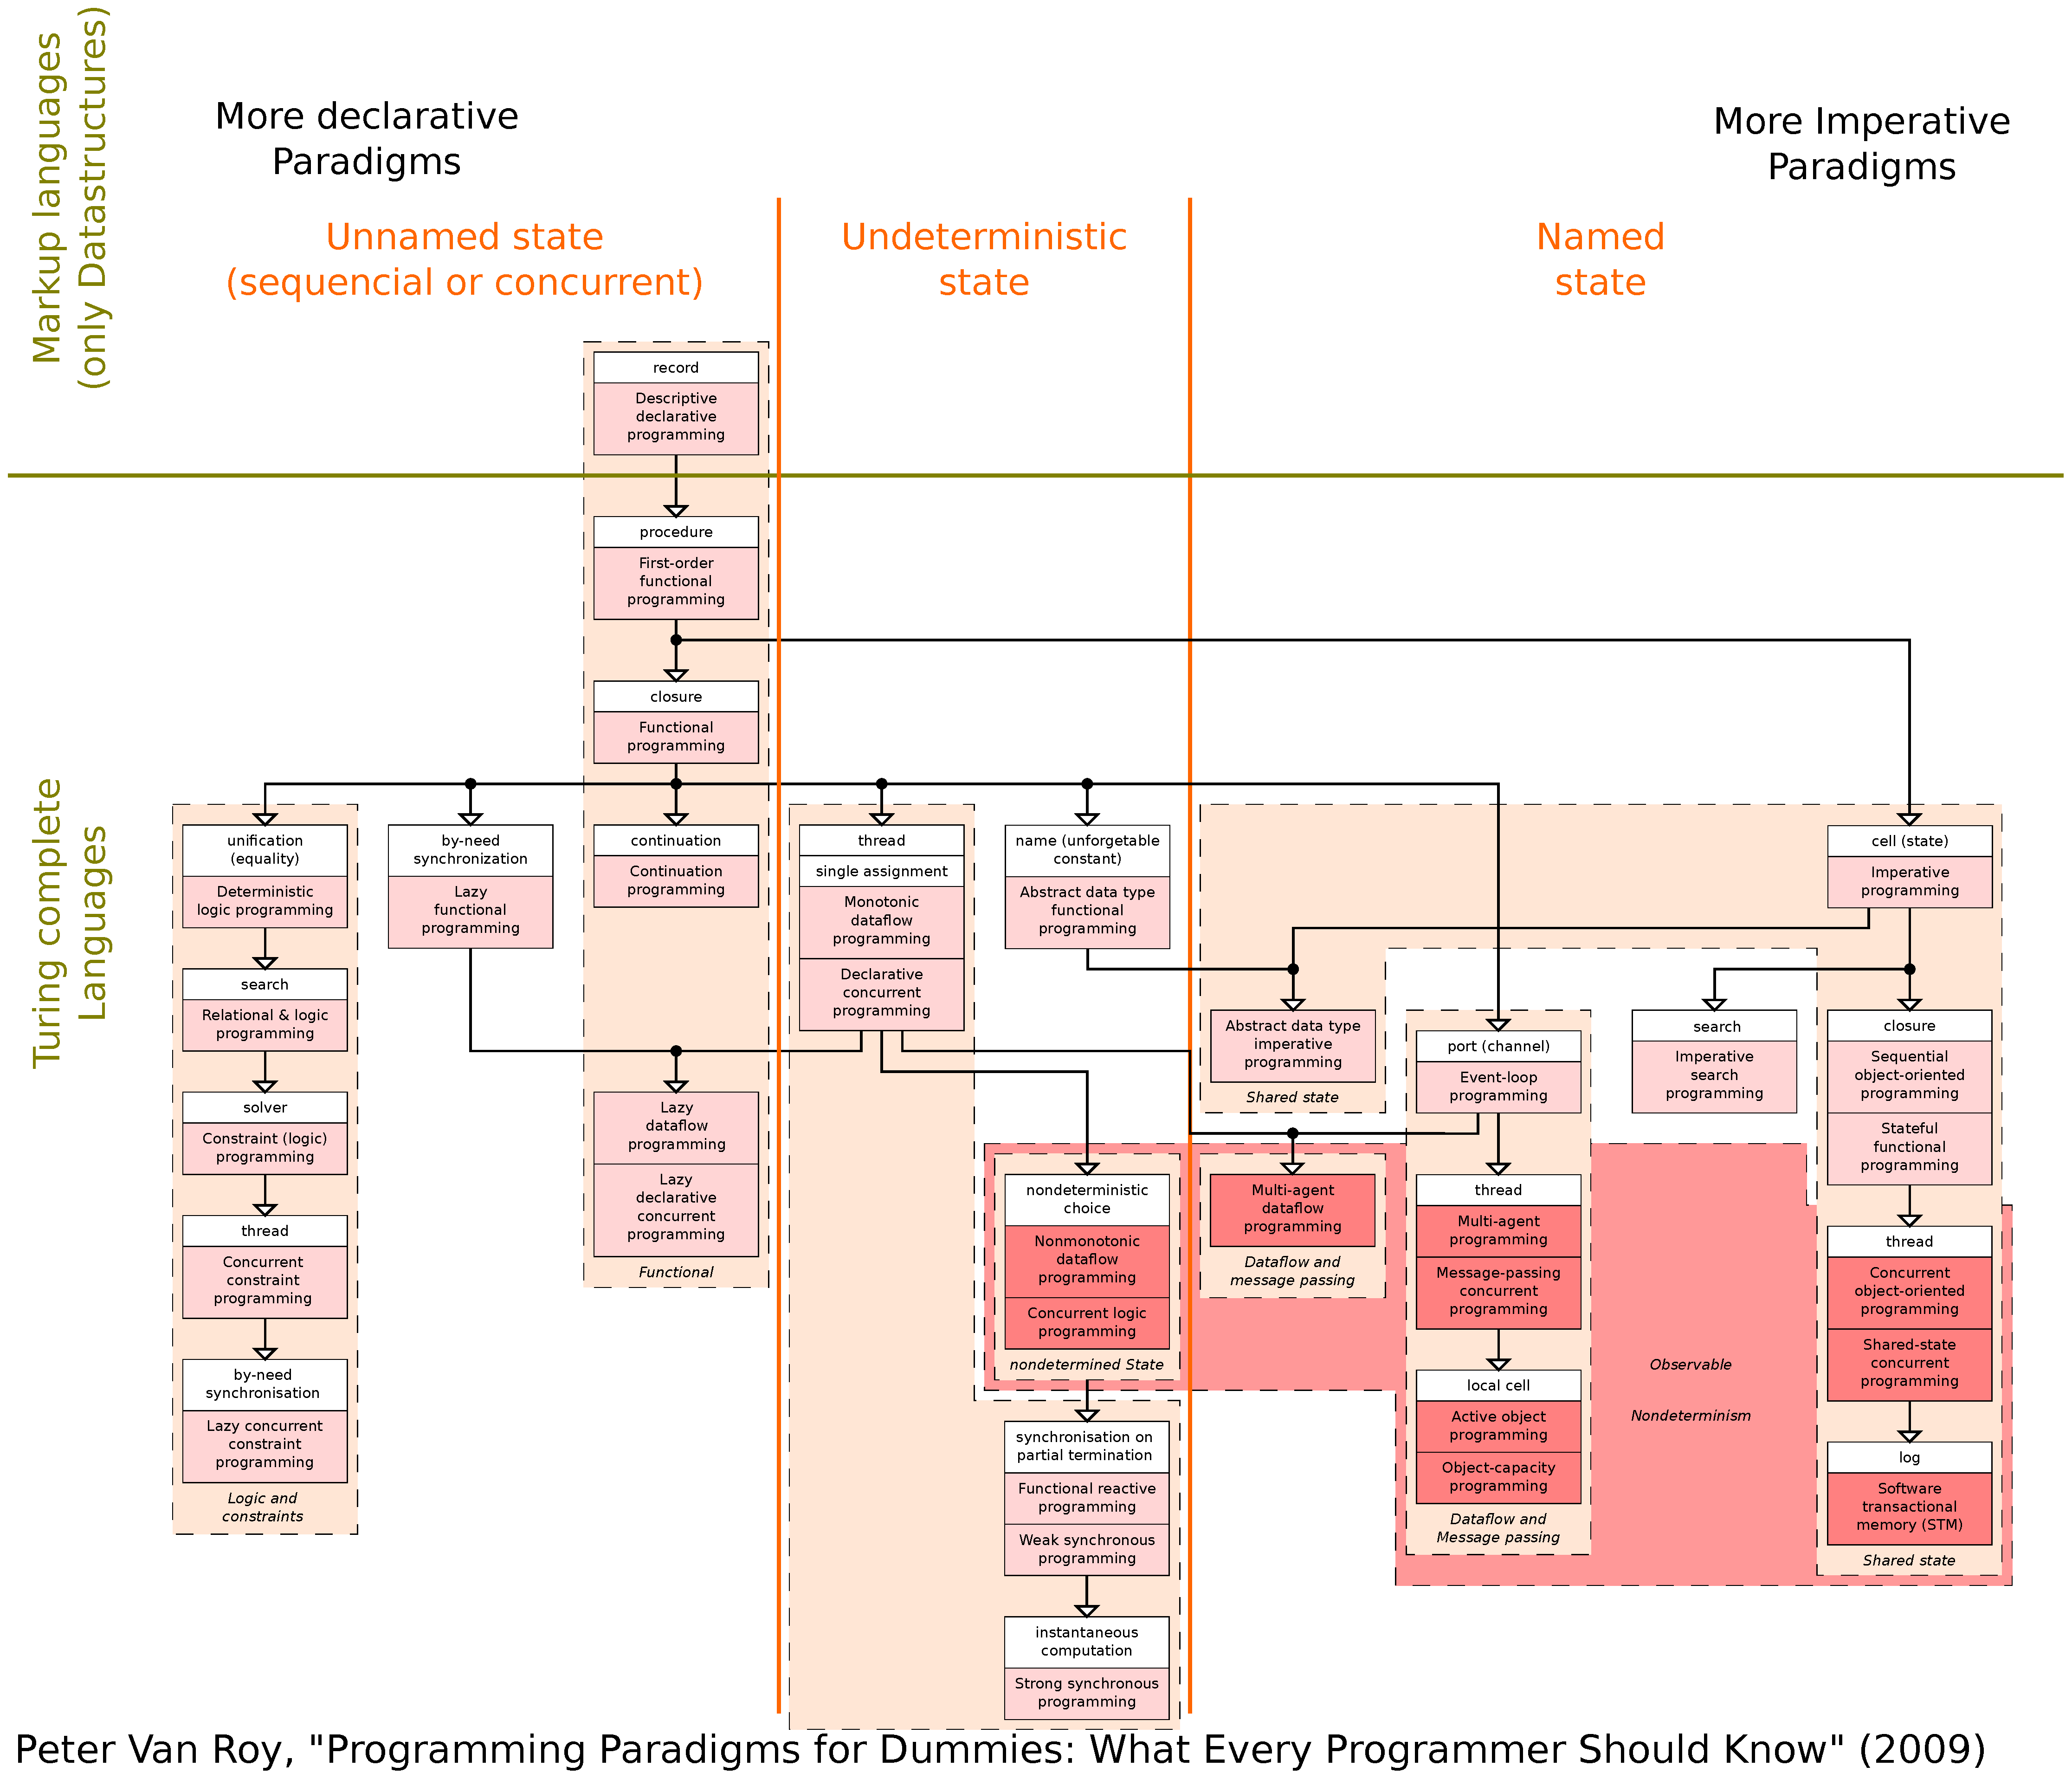
\includegraphics[scale=0.13]{lecture1_programming_paradigms.eps}
\end{frame}

\begin{frame}
\frametitle{Функциональное программирование}
\begin{itemize}
    \item Значения лучше переменных.
    \begin{itemize}
        \item Переменная даёт имя значению или функции, а не адресу в памяти.
        \item Переменные неизменяемы.
        \item Типы данных неизменяемы.
    \end{itemize}
    \item Выражения лучше инструкций.
    \begin{itemize}
        \item Аналоги \lstinline|if|, \lstinline|try-catch| и т.д. "--- выражения.
    \end{itemize}
    \item Функции как в математике (следующий слайд)
\end{itemize}
\end{frame}


\begin{frame}
\frametitle{Функциональное программирование}
\begin{itemize}
    \item Функции как в математике\pause
    \begin{itemize}
        \item Чистые функции: аргументу соответствует результат, а всё прочее от лукавого.
        \begin{itemize}
            \item Нет побочных эффектов (ввода-вывода, обращения к внешней памяти, не связанной с аргументом, и т.д.)
            \item При одинаковых аргументах результаты такой функции одинаковы
        \end{itemize}
        \item Функции являются значениями (функции первого класса)
        \item Функции часто принимают и возвращают функции (функции высших порядков)
    \end{itemize}
    \pause
    \item Опора на математические теории: лямбда-исчисление, теория типов, теория категорий
\end{itemize}
\end{frame}

\begin{frame}
\frametitle{Языки ФП}
\begin{itemize}
    \item семейство Lisp: первый ФП-язык и один из первых языков высокого уровня вообще
    \item Erlang и Elixir: упор на многозадачность (модель акторов), надёжность
    \item Scala, Kotlin, F\#: гибриды с ООП для JVM и для CLR
    \item Purescript, Elm, Ur/Web: для веба
    \item Семейство ML: OCaml, SML, F\#
    \pause
    \item \textbf{Haskell:}
    \begin{itemize}
        \item Чисто функциональный
        \pause
        \item Строго статически типизированный (с очень мощной и выразительной системой типов)
        \pause
        \item Ленивый
    \end{itemize}
\end{itemize}
\end{frame}

\begin{frame}[fragile]
\frametitle{Язык Haskell: начало}
\begin{itemize}
    \item Установите Haskell Platform (\url{https://www.haskell.org/platform/})
    \item Запустите WinGHCi (или просто GHCi)
    \item Это оболочка или REPL (Read-Eval-Print loop)
    \begin{itemize}
        \item Read: Вы вводите выражения Haskell (и команды GHCi)
        \item Eval: GHCi вычисляет результат
        \item Print: и выводит его на экран
    \end{itemize}
    \item Пример:
\begin{lstlisting}[breaklines]
GHCi, version 8.2.2: http://www.haskell.org/ghc/  :? for help
Prelude> 2 + 2
4
Prelude> :t True -- команда GHCi
True :: Bool
\end{lstlisting}
\end{itemize}
\end{frame}

\begin{frame}[fragile]
\frametitle{Язык Haskell: начало}
\begin{itemize}
    \item \lstinline|2 + 2|, \lstinline|True| "--- выражения
    \item \lstinline|4|, \lstinline|True| "--- значения
    \item \lstinline|Bool| "--- тип
    \pause
    \item Значение "--- \enquote{вычисленное до конца} выражение.
    \item Тип (статический) "--- множество значений и выражений, построенное по таким правилам, что компилятор может определить типы и проверить отсутствие ошибок в них без запуска программы.
    \item От типа зависит то, какие операции допустимы:
\begin{lstlisting}[basicstyle=\ttfamily\small]
Prelude> True + False

<interactive>:12:1: error:
No instance for (Num Bool) arising from a use of '+'
In the expression: True + False
In an equation for 'it': it = True + False
\end{lstlisting}
\item Это ошибка компиляции, а не выполнения.
\end{itemize}
\end{frame}

\begin{frame}[fragile]
\frametitle{Вызов функций}
\begin{itemize}
    \item Вызов (применение) функции пишется без скобок: \lstinline|f x|, \lstinline|foo x y|. 
    \item Скобки используются, когда аргументы "--- сложные выражения: \lstinline|f (g x)|
    \item И внутри сложных выражений вообще.
    \item Бинарные операторы (как \lstinline|+|) это просто функции с именем из символов вместо букв и цифр.
    \begin{itemize}
        \item Можно писать их префиксно, заключив в скобки: \lstinline[breaklines=false]|(+) 2 2|.
        \item А любую функцию двух аргументов с алфавитным именем можно писать инфиксно между обратными апострофами:
        \lstinline|4 `div` 2|.
        \item Единственный небинарный оператор "--- унарный \lstinline|-|.
    \end{itemize}
    \item Названия переменных и функций начинаются со строчной буквы (кроме операторов).
\end{itemize}
\end{frame}

\begin{frame}[fragile]
\frametitle{Определение функций и переменных}
\begin{itemize}
    \item Определение функции выглядит так же как вызов:
\begin{lstlisting}[breaklines]
название параметр1 параметр2 = значение
название = значение -- переменная
\end{lstlisting}
    \item Тело функции это не блок, а одно выражение (но сколь угодно сложное).
    \item В GHCi перед определением нужен \lstinline|let|, в отличие от кода в модулях:
\begin{lstlisting}
Prelude> let x = sin pi
Prelude> x !\pause!
1.2246063538223773e-16
Prelude> let square x = x * x
Prelude> square 2
4
\end{lstlisting}
\end{itemize}
\end{frame}

\begin{frame}[fragile]
\frametitle{Базовые типы}
\begin{itemize}
    \item Названия типов всегда с заглавной буквы.
    \item \lstinline|Bool|: логические значения \lstinline|True| и \lstinline|False|.
    \item Целые числа:
    \begin{itemize}
        \item \lstinline|Integer|: неограниченные (кроме размера памяти);
        \item \lstinline|Int|: машинные\footnote{по cтандарту минимум 30 бит, но в GHC именно 32 или 64 бита}, \lstinline|Word|: машинные без знака;
        \item \lstinline|Data.{Int.Int/Word.Word}{8/16/32/64}|: фиксированного размера в битах, со знаком и без.
    \end{itemize}
    \item \lstinline|Float| и \lstinline|Double|: 32- и 64-битные числа с плавающей точкой, по стандарту IEEE-754.
    \item \lstinline|Character|: символы Unicode.
    \item \lstinline|()|: \enquote{Единичный тип} (unit) с единственным значением \lstinline|()|.
\end{itemize}
\end{frame}

\begin{frame}[fragile]
\frametitle{Тип функций и сигнатуры}
\begin{itemize}
    \item Типы функций записываются через \lstinline|->|. Например, \lstinline|Int -> Char| это тип функции из \lstinline|Int| в \lstinline|Char|.
    
    \item Для нескольких аргументов это выглядит как \pause\lstinline|Bool -> Bool -> Bool|.
    
    \item \lstinline|::| читается как \enquote{имеет тип}.
    
    \item Запись \lstinline|выражение :: тип| "--- \enquote{сигнатура типа}.
    
    \item При объявлении экспортируемой функции или переменной  сигнатура обычно указывается явно:
\begin{lstlisting}
foo :: Int -> Char
foo x = ...
\end{lstlisting}
    \item Компилятор обычно может вывести типы сам, но это защищает от \emph{непреднамеренного} изменения.
\end{itemize}
\end{frame}

\begin{frame}[fragile]
\frametitle{Арифметика}
\begin{itemize}
    \item Это упрощённая версия.
    \item Полное объяснение требует понятия, которое будет введено позже. 
    \item Например, команды \lstinline|:type 1| или \lstinline|:type (+)| дадут тип, который понимать пока не требуется. 
    \item То же относится к ошибкам вроде \lstinline[breaklines=false]|No instance for (Num Bool)...|\\ на более раннем слайде.
    \item Пока достаточно понимать, что есть несколько числовых типов.
    \item Они делятся на целочисленные (\lstinline|Int|, \lstinline|Integer|) и дробные (\lstinline|Float|, \lstinline|Double|).
\end{itemize}
\end{frame}

\begin{frame}[fragile]
\frametitle{Числовые литералы}
\begin{itemize}
    \item Числовые литералы выглядят, как в других языках: \lstinline|0|, \lstinline|1.5|, \lstinline|1.2E-1|, \lstinline|0xDEADBEEF|. 
    \item Целочисленные литералы могут иметь любой числовой тип, а дробные любой дробный.
    \item Но это относится \emph{только} к литералам. 
    \item Неявного приведения (например, \lstinline|Int| в \lstinline|Double|) в Haskell \emph{нет}. 
\end{itemize}
\end{frame}

\begin{frame}[fragile]
\frametitle{Приведение числовых типов}
\begin{itemize}
    \item Используйте \lstinline|fromIntegral| для приведения из любого целочисленного типа в любой числовой. Тип-цель можно указать явно:
\begin{lstlisting}
Prelude> let {x :: Integer; x = 2}
Prelude> x :: Double
<interactive>:22:1: error:
Couldn't match expected type 'Double' with actual type 'Integer' ...
Prelude> fromIntegral x :: Double
2.0
\end{lstlisting}    
    \item А может выводиться из контекста:
\begin{lstlisting}
Prelude> :t fromIntegral 2 / (4 :: Double)
fromIntegral 2 / (4 :: Double) :: Double
\end{lstlisting}    
\end{itemize}
\end{frame}

\begin{frame}[fragile]
\frametitle{Приведение числовых типов}
\begin{itemize}
    \item \lstinline|toInteger| переводит любой целочисленный тип \\в \lstinline|Integer|.
    \item \lstinline|fromInteger| "--- наоборот. Если аргумент слишком велик, возвращает значение по модулю:
    \begin{lstlisting}
Prelude> fromInteger (2^64) :: Int
0
\end{lstlisting}
    \item \lstinline|toRational| и \lstinline|fromRational| "--- аналогично для \lstinline|Rational| и дробных типов.
    \item \lstinline|ceiling|, \lstinline|floor|, \lstinline|truncate| и \lstinline|round| "--- из дробных типов в целочисленные.
\end{itemize}
\end{frame}

\begin{frame}[fragile]
\frametitle{Арифметические операции}
\begin{itemize}
    \item Операции \lstinline|+|, \lstinline|-|, \lstinline|*| "--- как обычно (унарного \lstinline|+| нет).
    \item \lstinline|/| "--- деление \emph{дробных} чисел.
    \begin{itemize}
        \item Использование \lstinline|/| для целых чисел даст ошибку \lstinline|No instance... arising from a use of '/'|. \\Нужно сначала использовать \lstinline|fromIntegral|.
    \end{itemize}        
    \item \lstinline|div| "--- деление нацело
    \item \lstinline|mod| "--- остаток
    \item
\lstinline|quot| и \lstinline|rem| тоже, но отличаются от них поведением на отрицательных числах.
    \item \lstinline|^| "--- возведение любого числа в неотрицательную  целую степень. 
   \item \lstinline|^^| "--- дробного в любую целую. 
   \item \lstinline|**| "--- дробного в степень того же типа.
\end{itemize}
\end{frame}

\begin{frame}[fragile]
\frametitle{Операции сравнения и\\логические операции}
\begin{itemize}
    \item Большинство операций сравнения выглядят как обычно: \lstinline|==|, \lstinline|>|, \lstinline|<|, \lstinline|>=|, \lstinline|<=|.
    \item Но $\neq$ обозначается как \lstinline|/=|.
    \item Функция \lstinline|compare| возвращает \lstinline|Ordering|: тип с тремя значениями \lstinline|LT|, \lstinline|EQ| и \lstinline|GT|.
    \item Есть функции \lstinline|min| и \lstinline|max|.
    \item[]
    \item \enquote{и} это \lstinline|&&|, а \enquote{или} "--- \lstinline!||!, как обычно. 
    \item \enquote{не} "--- \lstinline|not|.
\end{itemize}
\end{frame}

%\begin{frame}
%    \href{run:./lecture2.pdf}{\beamergotobutton{Следующая лекция}}
%\end{frame}
\end{document}